%%
%%  chapter03.tex - Obstacle Detection and Planning for Autonomous Vehicles based on Computer Vision Techniques
%%
%%  Copyright 2014 Néstor Morales <nestor@isaatc.ull.es>
%%
%%  This work is licensed under a Creative Commons Attribution 4.0 International License.
%%

\graphicspath{{./images/chapter03/bmps/}{./images/chapter03/vects/}{./images/chapter03/}}

\chapter{Evaluation of stereo 3D reconstruction algorithms}\label{ch:chapter03}

Environment mapping is one of the most critical tasks in the development of \ac{ADAS} and stereo vision has been widely used to accomplish it. However, there are very few datasets that allow assessing the performance of a specific method in a real world application. Most datasets have been created in controlled conditions, thus neglecting scenarios that are impossible to reproduce in a laboratory. In this paper, we present the results of the evaluation of three different dense reconstruction algorithm implementations using a number of well-known strategies that represent different trade-offs in terms of cost, set up time and accuracy. In our tests, we evaluated two variants of the \acf{SGM} algorithm, and the \acf{ELAS} method, as well as different combinations of additional filters in order to assess their influence on the final behavior of the algorithms.

In this chapter, we will compare the performance level of some state-of-the-art stereovision-based 3D mapping algorithms in automotive scenarios, using both evaluation sets available in literature and data specifically collected from a dedicated recording platform. One of the algorithms will also be analyzed in greater detail, and a number of variations will be tested in order to determine an improved configuration.

\section{Experimental Setup}\label{ch:chapter03_01}

Real world scenarios come with little or no data to use as ground-truth, so one solution \cite{Morales2011, Geiger2012} is to use a high-end \ac{LIDAR} unit\footnote{\url{http://velodynelidar.com/lidar/hdlproducts/hdl64e.aspx}} to directly map the area surrounding the vehicle: depth measurements usually have centimeter-level accuracy over the range 5-100\,m, and produce reasonably dense maps, with up to 64 horizontal scanning planes. Another option is to exploit a prior over the data-set, such as the presence of freespace in front of a manually driven vehicle \cite{Steingrube2009} to detect wrongly reconstructed points (false stereo correspondences) over an extended period of time. Finally, a virtual view synthesized from the reconstructed environment geometry can be compared with the actual data recorded by a third, suitably positioned physical camera \cite{Morales2011, Morales2009}.
In this evaluation the algorithms have been tested using all the mentioned approaches, in order to get a better understanding of their behavior in real-world applications. Some of the tests have been carried out on data acquired using the vehicle depicted in figure \ref{fig:cp03_VIAC}, which has been equipped with a forward-looking Point Grey Bumblebee® XB3-13S2C color camera with 3.5\,mm optics working at a resolution of 1280$\times$960 pixels. The imaging system is synchronized to a SICK LD-MRS-400001 4-plane LIDAR unit running at 12.5\,Hz, with an angular resolution of 0.125$^\circ$ and a field of view of 85$^\circ$, integrated in the front bull-bar. GPS and INS information are provided by a Topcon AGI-3 unit, and are used to predict the vehicle trajectory.

\begin{figure}[thpb]
      \centering
      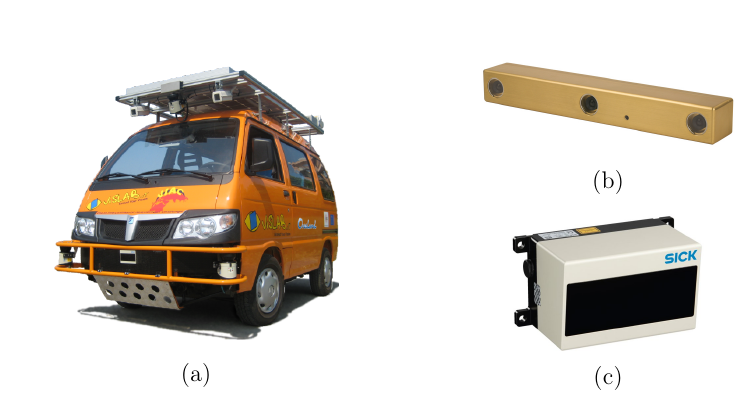
\includegraphics[width=\textwidth, trim=0 0 0 40,clip]{viac}
      \caption{ The recording platform. Data has been collected using one of the electric vans a) which had been set up in 2010 to take part to the VisLab Intercontinental Autonomous Challenge (VIAC) \cite{Broggi2010VIAC}. b) The imaging unit  is synchronized to a LIDAR c) working at a frequency of 12.5\,Hz. }      
      \label{fig:cp03_VIAC}
\end{figure}

A test sequence has been recorded in a mixed suburban and country environment. The data-set has been acquired along a 15\,Km loop around the University of Parma campus surroundings; the recording session took place at around 13:14 on a sunny September day, and the scenarios include narrow country roads (\ref{fig:cp03_countryRoad}), small downtowns(\ref{fig:cp03_downtown}), intersections (\ref{fig:cp03_intersection}) and motorways (\ref{fig:cp03_motorway}).

\begin{figure*}[h!]
        \centering
        \begin{subfigure}[b]{0.45\textwidth}
	  \begin{tabular}{c}
	    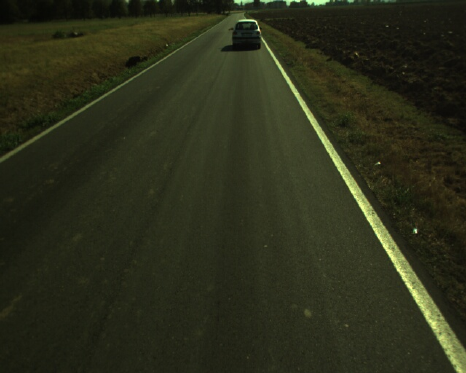
\includegraphics[width=\textwidth]{countryRoad}
	  \end{tabular}
	  \caption{}\label{fig:cp03_countryRoad}
        \end{subfigure}% 
        ~
        \begin{subfigure}[b]{0.45\textwidth}
	  \begin{tabular}{c}
	    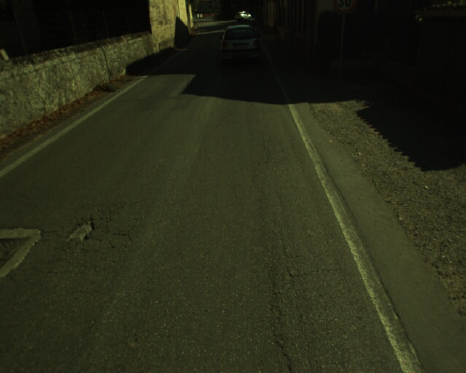
\includegraphics[width=\textwidth]{downtown}
	  \end{tabular}
	  \caption{}\label{fig:cp03_downtown}
        \end{subfigure}%       
        
        \centering
        \begin{subfigure}[b]{0.45\textwidth}
	  \begin{tabular}{c}
	    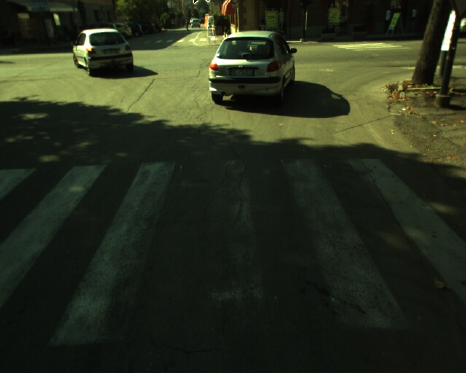
\includegraphics[width=\textwidth]{intersection}
	  \end{tabular}
	  \caption{}\label{fig:cp03_intersection}
        \end{subfigure}% 
        ~
        \begin{subfigure}[b]{0.45\textwidth}
	  \begin{tabular}{c}
	    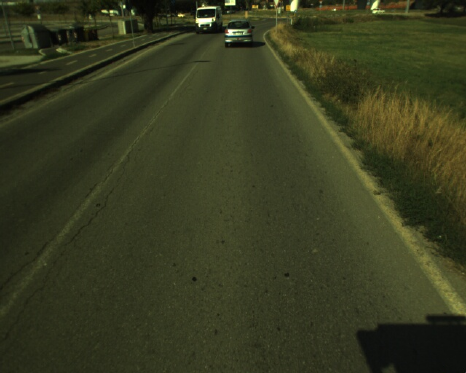
\includegraphics[width=\textwidth]{motorway}
	  \end{tabular}
	  \caption{}\label{fig:cp03_motorway}
        \end{subfigure}%       
        \caption{Samples of the recorded data.}\label{fig:cp03_samples}
\end{figure*}

\subsection{Dense \ac{LIDAR}-based ground truth}\label{ch:chapter03_01_01}

As a reference, the test data-set available at \footnote{\url{http://www.cvlibs.net/datasets/kitti}} has been used. Ground truth for a given frame is obtained by registering 5 consecutive frames before and after the one selected and accumulating the resulting point clouds; ambiguous regions such as windows and fences are manually removed, and finally the corresponding disparity map is computed using calibration information (see figure \ref{fig:cp03_lidarGT}).

\begin{figure*}[h!]
        \centering
        \begin{subfigure}[b]{\textwidth}
	  \begin{tabular}{c}
	    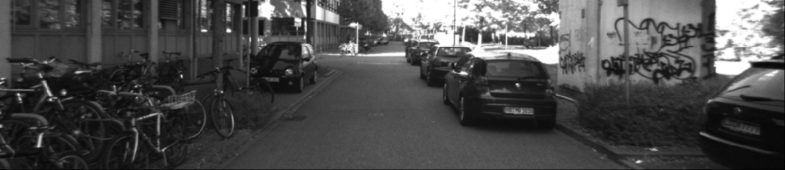
\includegraphics[width=\textwidth]{lidarGTOriginal}
	  \end{tabular}
	  \caption{The original image.}\label{fig:cp03_lidarGTOriginal}
        \end{subfigure}% 
        
        \begin{subfigure}[b]{\textwidth}
	  \begin{tabular}{c}
	    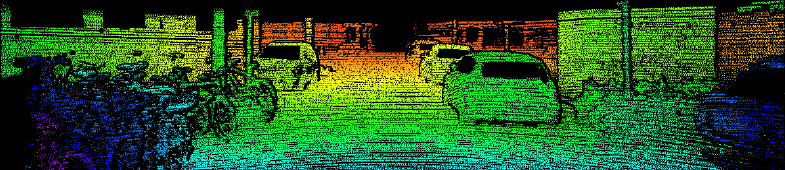
\includegraphics[width=\textwidth]{lidarGT}
	  \end{tabular}
	  \caption{The LIDAR-generated ground truth disparity map.}\label{fig:cp03_lidarGT}
        \end{subfigure}%       
        
        \begin{subfigure}[b]{\textwidth}
	  \begin{tabular}{c}
	    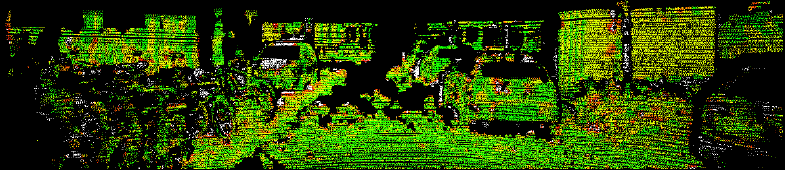
\includegraphics[width=\textwidth]{lidarErrMap}
	  \end{tabular}
	  \caption{The error map, with colors spanning from green (error = 0\,px) to red (error = 3\,px). White pixels correspond to areas with a reconstruction error greater than 3\,px.}\label{fig:cp03_lidarErrMap}
        \end{subfigure}%    
        
        \caption{\ac{LIDAR}-based ground truth example.}\label{fig:cp03_lidarGT}
\end{figure*}

However, in this work scores are being computed in a slightly different manner, since the original metrics did not look completely fair. In particular:
\begin{itemize}
\item only non-occluded, computed pixels are being considered. The original benchmark also gives statistics after linear interpolation of missing values, with the aim of making sparse and semi-dense methods comparable to dense ones; however, such an approximation is hardly optimal, and this reflects on unfairly worsened error metrics for non-dense algorithms.
\item average errors have been computed considering only the values below the endpoint error, and not all the values, in order to get a better estimate of the behavior for relevant pixels.
\item statistics for each frame are being considered, not just their average over an entire sequence. To make the data easier to understand, it will be plotted in a graph with the independent variable (x-axis) representing the measured value, and the dependent one (y-axis) the percentage of frames falling below it. Better-performing algorithms are those with a lower x value for a given frame percentage (e.g. y = 90\%).
\end{itemize}

\subsection{False correspondences estimation}\label{ch:chapter03_02}

This benchmark is an adaptation of one of the techniques described in \cite{Steingrube2009}: when driving manually, a safety distance of about 1\,s is usually kept from a leading vehicle; this means that a (speed-dependent) volume of free space is present at all times in front of the ego-vehicle, and any reconstructed point falling within said area must be considered as an erroneous estimate, as shown in figure \ref{fig:cp03_fc}. The false correspondences percentage $m_{fc} = 100 \times N_{fc} / N$ is then the ratio of points inside the object-free volume with respect to the total number of 3D points.

\begin{figure}[h!]
\centering
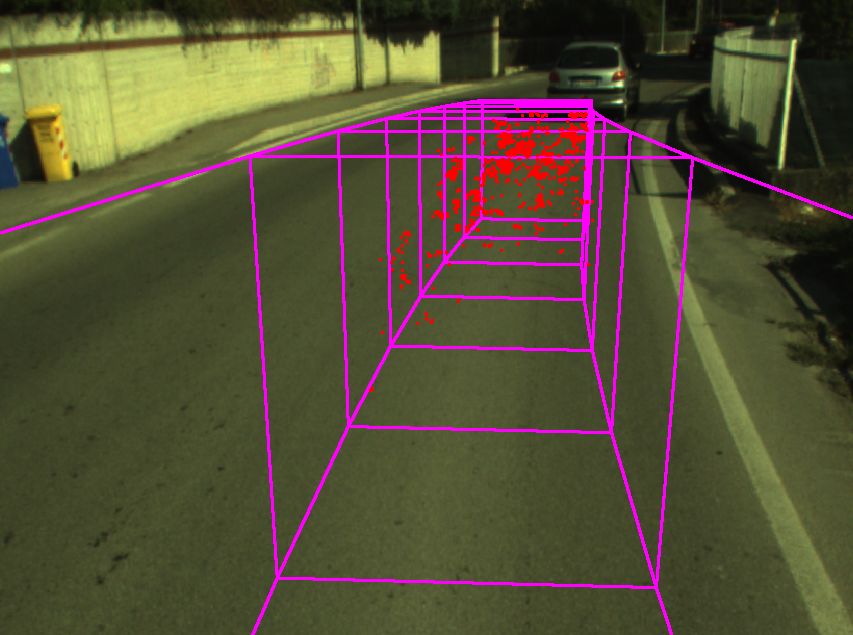
\includegraphics{fc}
\caption{False correspondences estimation example. In pink, the object-free volume which is present in front of the vehicle and, in red, the points falling within said area, produced by false matches.}\label{fig:cp03_fc}
\end{figure}

\subsection{Normalized cross correlation}\label{ch:chapter03_03}

The approaches introduced so far have some limitations: LIDAR-based ground truth still takes time to be produced, so it cannot be provided for large data-sets, while leading vehicle measurement can be easily performed even on long sequences, but it is an indirect performance metric, albeit a relevant one. As an alternative, the use of a third camera \cite{Morales2009}, as illustrated in figure \ref{fig:cp03_trinocular_setup}, allows to directly compare a reconstructed view with the actual images without any manual intervention. 

\begin{figure}[h!]
\centering
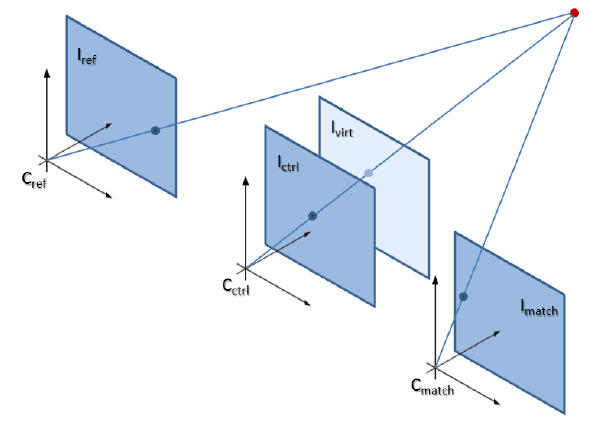
\includegraphics{trinocular_setup}
\caption{Trinocular camera setup for stereo evaluation. The reference and match cameras ($C_{ref}$ and $C_{match}$ respectively) are used to produce a virtual image $I_{virt}$ in the control camera’s reference system that can be compared to the actual recorded image $I_{ctrl}$.}\label{fig:cp03_trinocular_setup}
\end{figure}
   
The computed disparity map is used to transform image pixels taken from the reference camera into control camera coordinates, thus effectively creating a virtual image (figure \ref{fig:cp03_lidarGTOriginal}) that can be compared with that recorded by the control camera (figure \ref{fig:cp03_lidarGT}) to produce a cross correlation map (figure \ref{fig:cp03_lidarErrMap}). 

\begin{figure*}[h!]
        \centering
        \begin{subfigure}[b]{0.3\textwidth}
	  \begin{tabular}{c}
	    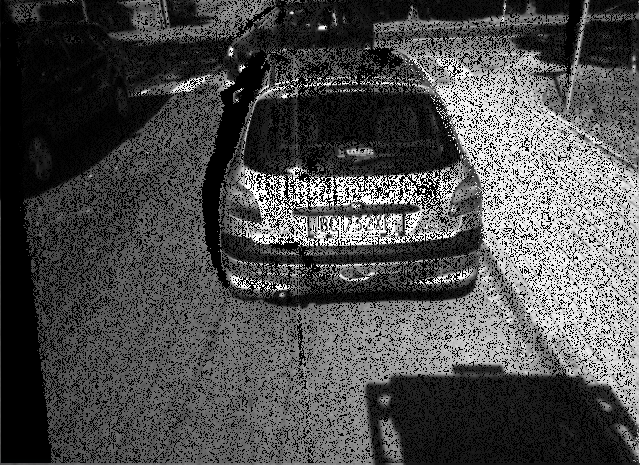
\includegraphics[width=\textwidth]{reprojection}
	  \end{tabular}
	  \caption{}\label{fig:cp03_lidarGTOriginal}
        \end{subfigure}% 
        ~
        \begin{subfigure}[b]{0.3\textwidth}
	  \begin{tabular}{c}
	    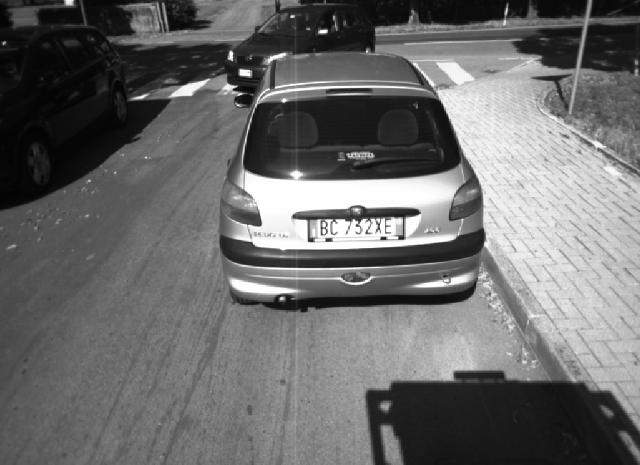
\includegraphics[width=\textwidth]{leftNCC}
	  \end{tabular}
	  \caption{}\label{fig:cp03_lidarGT}
        \end{subfigure}%       
        ~
        \begin{subfigure}[b]{0.3\textwidth}
	  \begin{tabular}{c}
	    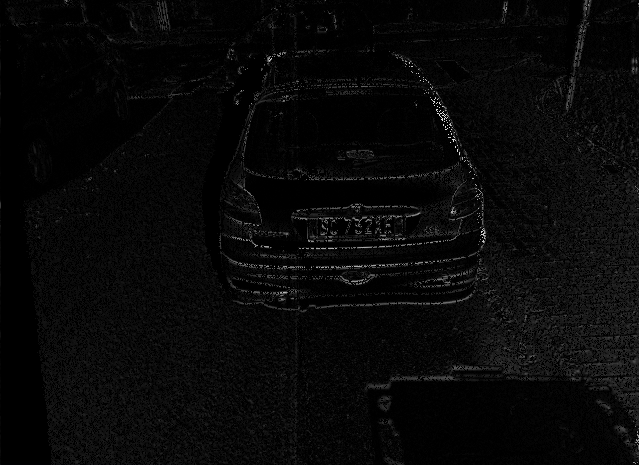
\includegraphics[width=\textwidth]{ncc}
	  \end{tabular}
	  \caption{}\label{fig:cp03_lidarErrMap}
        \end{subfigure}%    
        
        \caption{TODO. Cambiar labels, también}\label{fig:cp03_lidarGT}
\end{figure*}

However, care must be taken to ensure that the results are meaningful: camera calibration is a source of error which must be kept to a minimum, and the occasional presence of obstacles within the object-free volume must be handled as well. The chosen metric is the Normalized Cross Correlation (NCC), computed as:

\begin{equation}\label{eq:cp03_NCC}
NCC(I_v,I_c) = {{{1} \over {\Omega}}  \sum_{(x,y) \in \Omega} {{[I_c(x,y)-\mu_c][I_v(x,y)-\mu_v]} \over {\sigma_c \sigma_v}}}
\end{equation}

where $\Omega$ is the subset of all pixels having a valid disparity; $\mu_c$, $\mu_v$, $\theta_c$, $\theta_v$ are the mean and standard deviation of the control and virtual images respectively.
It is worth noticing that in \cite{Morales2011} it is suggested a configuration with the reference and match camera lying 30\,cm apart, and the control camera at 50 cm from the reference camera; however, the recording platform used in this work uses much shorter distances (24 and 12\,cm respectively), as illustrated in the next section, since it has been equipped with a pre-calibrated trinocular camera. Moreover, in this study the control camera has been kept in between the reference and match cameras. This layout makes the virtual and control images look more similar, and could potentially yield to improved NCC scores due to the lower disparity ranges encountered. However, factory calibration is still significantly better than what can be currently achieved with lab equipment, and the resulting
accuracy improvement has been deemed more relevant than the quantization introduced by the disparity range reduction.

\section{Calibration}\label{ch:chapter03_02}

\subsection{LIDAR to camera calibration}\label{ch:chapter03_02_01}

In order to obtain meaningful results, the LIDAR unit has been used to detect the presence of real obstacles inside the free space area. To do that, it is necessary to know the relative position between the stereo rig and the laser-scanner. This calibration procedure starts with an initial rough alignment step; after that, easily recognizable LIDAR points are manually associated to the corresponding image pixel. The accuracy of each association is constrained by several factors, such as the LIDAR angular resolution and the ambiguity of the candidates to be selected as correspondences in the image. However, with this method, a large number of samples can be quickly collected over different frames, and used together in a non-linear Maximum-Likelihood minimization framework. As a non-linear solver, the Levenberg-Marquardt approach has been chosen.

In order to obtain meaningful results for the false stereo correspondences test described before, the LIDAR unit has been used to detect the occasional presence of close preceding vehicles within the defined free space area. To perform this operation it is necessary to measure the relative positioning of the stereo rig and the laser-scanner, which is challenging, given the relatively small amount of data that the available 4-plane LIDAR produces.
The calibration procedure starts with an initial rough alignment step; after that, easily recognizable LIDAR points are manually associated to the corresponding image pixel. The accuracy of each association is constrained by several factors, such as the LIDAR angular resolution, and the ambiguity arising by the limited number of scanning planes hitting each surface; however, a large number of samples can be quickly collected over different frames, and used together in a non-linear Maximum-Likelihood minimization framework, using as a cost function:

\begin{equation}\label{eq:cp03_ML}
\underset{[R|t]}{\arg\min} \sum_{i} \lVert p_i - K[R|t] w_i \rVert^2
\end{equation}

with $[R|t]$ being the unknown rototranslation matrix to estimate, $p$ a given 2D (undistorted) image pixel and $w$ the corresponding world point. Assuming to operate under a pin-hole camera model, $K$ is the camera projection matrix. As a non-linear solver, the Levenberg-Marquardt (\cite{Levenberg1944}) approach has been chosen, given its robustness an relatively fast convergence times.

\subsection{Camera-to-camera calibration}\label{ch:chapter03_02_02}

In order to perform the test described in section \ref{ch:chapter03_03} with the hardware setup in use the relative positioning between all of the cameras has to be computed, since Point Grey Bumblebee\textregistered{} XB3-13S2C cameras only provide combined rectification and dedistorsion look-up tables for left-right and center-right baselines.
Let $P_{mw}$ and $P_{ms}$ be two homogeneous disparity points on the right (match, see figure \ref{fig:cp03_trinocular_setup}) camera in the wide and short reference systems respectively:

\begin{align}\label{eq:cp03_dispPoints}
& P_{mw} = (u_{rw} - d_{rw}, v_{rw}, -d_{rw}, 1) \nonumber \\
& P_{ms} = (u_{rs} - d_{rs}, v_{rs}, -d_{rs}, 1)
\end{align}

then there exist a 3D homography matrix H so that $P_{ms} = HHP_{mw}$ , in the form:

\begin{equation}\label{eq:cp03_homographyMatrix}
H = Q_s^{-1} \left[ \begin{array}{cc}
R & t \\
0 & 1 \end{array} \right] Q_w
\end{equation}

, where $Q_s^{-1}$ is the $4 \times 4$ matrix that transforms from camera coordinates to rectified image coordinates in the short baseline, and $Q_w$ is the $4 \times 4$ matrix that transforms from rectified image coordinates to camera coordinates in the wide baseline. The $R$ and $t$ terms in equation \ref{eq:cp03_homographyMatrix}, instead, represent the rotation and translation components that align the two baselines. The unknown rotation $R$ is very close to the identity since the three cameras are almost physically aligned, and a linear solver has proved enough to directly estimate the terms of the $H$ matrix, using feature-based correspondences to generate the needed pixelwise associations. Once $H$ is known, the luminance value $I(P_{rw})$ of each point with a known disparity value is used to build the virtual image, by projecting it into coordinates $(u_{rs} , v_{rs})$, exploiting equation \ref{eq:cp03_dispPoints}.

\section{Algorithms}\label{ch:chapter03_03}

In order to have a broad range of performance statistics, three different dense reconstruction algorithm implementations have been tested. The first two are both based on the so-called Semi-Global Matching approach (in short, SGM) first presented in \cite{Hirschmuller2005}, albeit exploiting different metrics for cost volume initialization, while the latter \cite{Geiger2011} matches sparse features in the left and right images to restrict the search range of a local window-based approach.

\subsection{Semi-Global Matching}\label{ch:chapter03_03_01}

The Semi-Global Matching approach aims at identifying the disparity map $D$ that minimizes the energy function

\begin{equation}\label{eq:cp03_SGM_energy}
E(D) = E_{data}(D) + E_{smooth}(D)
\end{equation}

with $E_{data}(D)$ representing the pixel-wise matching cost and Esmooth(D) a smoothness constraint.

In particular, the $E_{data}(D)$ term is the sum of all pixel matching costs $C$ for the disparities of $D$:

\begin{equation}\label{eq:cp03_SGM_energy_data}
E_{data}(D) = \sum_p C(p, D_p)
\end{equation}

while the $E_{smooth}$ term adds a small penalty $P_1$ to all pixels $q$ in the neighborhood $N_p$ of $p$, for which the disparity varies from $p$ by one, and a higher penalty $P_2$ if the difference is greater:

\begin{align}\label{eq:cp03_SGM_energy_smooth}
  E_{smooth} = & \sum_{q \in N_p} P_1 T[\lvert D_p - D_q \rvert = 1] \quad + \nonumber \\
	       & \sum_{q \in N_p} P_2 T[\lvert D_p - D_q \rvert > 1]
\end{align}

with

\begin{equation}\label{eq:cp03_SGM_energy_smooth_T}
 T[x] = \left\{ \begin{array}{ll}
         1 & \mbox{if $x$ is true}\\
         0 & \mbox{otherwise}
         \end{array} \right.
\end{equation}

Global optimization of $E(D)$ is a complex task (i.e. NP-complete), and currently intractable in real time; however, good results can be obtained by applying a dynamic programming strategy that computes the values of $E(D)$ along 1D paths from 8 directions towards each pixel. The costs $Lr'$ of each path $r$ are aggregated as described in equation \ref{eq:cp03_SGM_cost_Lr} for each pixel $p$ and disparity $d$:

\begin{align}\label{eq:cp03_SGM_cost_Lr}
L_r'(p,d) = C(p,d) + \min( & L_r'(p-r,d), \nonumber \\
	    & Lr'(p-r, d-1) + P_1, \nonumber \\
	    & Lr'(p-r,d+1)+P_1, \nonumber \\
	    & \min_i Lr'(p-r, i) + P_2)
\end{align}

The final disparity value for each pixel is then determined by a winner-takes-all strategy applied to the values of $L_r'$.

\subsubsection{Census cost metric}\label{ch:chapter03_03_01_01}

Instead of using mutual information as the pixel-wise matching function, as it is done in the original work (\cite{Hirschmuller2005}), the Hamming distance of the Census transform of a $5 \times 5$ window cropped around each pixel has been computed, since it provides similar results (\cite{Hirschmuller2009}) while reducing the overall processing burden.

The Census transform of a window $W$ taken from an image $I$ and centered around a pixel $p$ is defined as:

\begin{align}\label{eq:cp03_census_transform}
census(I, p) = \underset{\bar{p} \in W}{\bigotimes} \xi(I(p), I(\bar{p}))
\end{align}

where $\bigotimes$ denotes concatenation, and $\xi(I(p), I(\bar{p}))$ is defined as:

\begin{equation}\label{eq:cp03_census_xi}
\xi(I_p, I_{\bar{p}}) = \left\{ \begin{array}{ll}
         1 & \text{if~} I_p < I_{\bar{p}}\\
         0 & \text{otherwise}
         \end{array} \right.
\end{equation}

Each position $C(p, d)$ of the cost volume is then initialized with the number of differing bits between the corresponding transformed values of the left and right images.

\subsubsection{Birchfield-Tomasi cost metric}\label{ch:chapter03_03_01_02}

The freely available OpenCV SGM implementation \footnote{\url{http://www.opencv.org}} (BT-SGM in the following) uses the Birchfield-Tomasi pixel dissimilarity metric \cite{Birchfield1998} to initialize the cost volume.

Let $I_L$ and $I_R$ be the 1D functions representing the intensity values along a given scan-line in the left and right images respectively, and $\hat{I}_L(x_L)$, $\hat{I}_R(x_R)$ the linearly interpolated functions between the sample points around $x_L$ and $x_R$. It is then possible to determine how well the intensity at $x_L$ fits into the linearly interpolated region surrounding $x_R$.

\begin{align}\label{eq:cp03_birchfield_tomasi_l_in_r}
\bar{d}(x_L, x_R, I_L, I_R) = \underset{x_R - {1 \over 2} \leq x \leq x_R + {1 \over 2}}{min} | I_L(x_L) - \hat{I}_R(x)|
\end{align}

and symmetrically:

\begin{align}\label{eq:cp03_birchfield_tomasi_r_in_l}
\bar{d}(x_R, x_L, I_R, I_L) = \underset{x_L - {1 \over 2} \leq x \leq x_L + {1 \over 2}}{min} | I_R(x_R) - \hat{I}_L(x)|
\end{align}

The dissimilarity between the pixels at $x_L$ and $x_R$ then becomes:

\begin{align}\label{eq:cp03_birchfield_tomasi}
d(x_L, x_R) = min \{ \bar{d}(x_L, x_R, I_L, I_R), \bar{d}(x_R, x_L, I_R, I_L) \}
\end{align}

and is used to initialize the cost volume for any given pixel and disparity value.


\subsection{Efficient Large-Scale Stereo Matching}\label{ch:chapter03_03_02}

This method, proposed in \cite{Geiger2011} and referred to as ELAS in the following is particularly suited for handling the high disparity ranges which can arise by using large baselines or very high resolutions images.

It exploits sparse, robustly matched control points to generate a 2D mesh via Delaunay triangulation, which in turn is leveraged to create a prior that is used to reduce the disparity search range for the remaining pixels. Said prior is formed by computing a piecewise linear function induced by the support point disparities and the triangulated mesh.

\subsection{Additional filters}\label{ch:chapter03_03_03}

A number of pre- and post-processing filters, and their combinations, have been tested in order to determine which would be the most effective in improving the quality metrics discussed previously:

\begin{itemize}
\item Gaussian filter. A 3$\times$3 Gaussian smoothing mask is applied to both gray-scale input images.
\item Sparse Census mask. Following \cite{Pantilie2012}, a sparse pattern is used to compute the Census transform of the input images.
\item Ternarized Census. In order to improve the amount of information about the local image structure encoded in the resulting images, the Census transform function has been modified to return three different symbols $(00, 01, 11)$, instead of just $0, 1$.
\item Hamming scores aggregation. As suggested in \cite{Pantilie2012}, a 5$\times$5 window centered around each pixel is used to preprocess each score in the input cube.
\item Uniqueness constraint. The ratio between the first and second minima of the aggregated cost function for a given pixel is used to determine whether a match is reliable or not: higher ratios correspond to a strong minimum, which is more likely to be correct.
\item Adaptive mean. An 8$\times$8 adaptive mean filter \cite{Geiger2011} is applied over the resulting disparity map $D$.
\item Despeckle filter. Small disparity image patches with values very different from their neighborhood are usually likely to correspond to wrong associations, so the strategy proposed in \cite{Hirschmuller2008} is used to identify and remove them.
\item Gap filter. Constant interpolation along 1D horizontal and vertical paths in the disparity image is performed in order to fill small ($\leq 3$\,px) areas with missing disparity values \cite{Geiger2011}.
\end{itemize}

Each filter has been tested individually against the Census-SGM baseline configuration, and three promising setups have been selected. Each setup has then been compared against other approaches, which also share some of the same filtering strategies, as detailed in Tab. \ref{table:cp03_algorithms}. For the BT-SGM and ELAS algorithms the setups suggested in \cite{Geiger2012} have been followed.

\begin{savenotes}
\begin{table}[h]
\begin{center}
\resizebox{\columnwidth}{!} {
\begin{tabular}{|l|c|c|c|c|c|}
 \cline{2-6}
 \multicolumn{1}{ c|}{} & \multicolumn{3}{ c| }{Census-SGM} &
 \multicolumn{1}{ c| }{\multirow{2}{*}{BT-SGM}} &
 \multicolumn{1}{ c| }{\multirow{2}{*}{ELAS}} \\ \cline{2-4}
 \multicolumn{1}{c|}{} & Config 1 & Config 2 & Config 3 & & \\ \cline{2-6}
 \hline \hline
 Gaussian filter & $\surd$ & $\surd$ & $\surd$ & - & - \\
 Sparse Census mask & - & - & - & - & - \\
 Ternarized Census & - & - & - & - & - \\
 Hamming scores aggregation  & - & - & - & - & - \\
 Uniqueness constraint & 10 & 20 & 20 & 10 & 15 \\
 Adaptive mean & $\surd$ & $\surd$ & $\surd$ & - & $\surd$ \\
 Despeckle filter & $\surd$ & $\surd$ & $\surd$ & $\surd$ & $\surd$ \\
 Gap filter & $\surd$ & $\surd$ & - & - & $\surd$ \\
 \hline \hline
 Other parameters & \multicolumn{3}{ |c }{$P_1=10$, $P_2=50$, L/R check} &
 \multicolumn{1}{ |c }{see \footnote{\url{http://www.cvlibs.net/datasets/kitti/eval\_stereo\_flow.php}}} &
 \multicolumn{1}{ |c| }{see \footnotemark[\value{footnote}]} \\
 \hline
\end{tabular}
}
\caption{Algorithm configurations}\label{table:cp03_algorithms}
\end{center}
\end{table}
\end{savenotes}

\section{Summary}\label{ch:chapter03_05}

The tests conducted so far have quantitatively confirmed how targeted filtering strategies can substantially reduce the amount of wrong pixels computed during stereo reconstruction, while also improving the results accuracy.

In particular, the Census-SGM configuration 2 described in section \ref{ch:chapter03_03_01_01} reduces the number of bad pixels by 7.5\% at the 90th percentile, while also improving the average error by 0.15\,px, making it the candidate of choice among those tested.

This evaluation also served to validate the strategies employed. While LIDAR-based ground truth (see section \ref{ch:chapter03_01_01}) is very effective at producing reliable statistics, it remains quite expensive to carry out, both in terms of the equipment required and of the manual post-processing that has to be performed to produce each frame.

As an alternative, the use of a prior on the vehicle movement (section \ref{ch:chapter03_02}) can be successfully exploited to identify a portion of the wrongly reconstructed points. The advantage of this approach is that it can be effectively used to evaluate the behavior of an algorithm on big data-sets, thus covering a broad range of environmental conditions. On the other hand, the portion of space that can be checked is limited to the area in front of a moving vehicle, which often times is the most critical, but nonetheless can introduce a bias in the resulting statistics.

The use of a third camera for evaluation (section \ref{ch:chapter03_03}) is conceptually appealing, but in practice has shown to produce poor results. Further testing will be needed to assess its real effectiveness in real-world scenarios. In the future, we expect to perform more experiments including more sequences with different atmospheric conditions like other hours in a day, as well as the use of different metrics to measure the similarity between the control camera and virtual images.

The algorithms shown here and their associated filters are used for a dense reconstruction of the world. However, in order to save computational costs, there are other approaches for 3D reconstruction of the environment of the vehicle which avoid the full reconstruction of the environment. In the next chapter, we will see one of these approaches, which is based on the Stixel World decribed by \cite{badino2009stixel}.
